\documentclass[a4paper,onesided,12pt]{report}
\usepackage{styles/fbe_tez}
\usepackage[utf8]{inputenc} % To use Unicode (e.g. Turkish) characters
\renewcommand{\labelenumi}{(\roman{enumi})}
\usepackage{amsmath, amsthm, amssymb}
 % Some extra symbols
\usepackage[bottom]{footmisc}
\usepackage{cite}
\usepackage{graphicx}
\usepackage{longtable}
\graphicspath{{figures/}} % Graphics will be here

\usepackage{multirow}
\usepackage{subfigure}
\usepackage{algorithm}
%\usepackage{algorithmic}
\usepackage{algpseudocode}
%\pagestyle{empty}
%\includeonly{introduction} % To only process the given file

\newtheorem{thm}{Theorem}[chapter]
\newtheorem{prop}[thm]{Proposition}
\newtheorem{lem}[thm]{Lemma}
\newtheorem{cor}[thm]{Corollary}
% COVER PAGE
\title{AIRFLOW ESTIMATION FROM RESPIRATORY SOUNDS}
\turkcebaslik{SOLUNUM SESLERİNDEN SOLUK AKIŞI KESTİRİMİ}
\degree{B.S., Electrical \& Electronics Engineering, Boğaziçi University, 2013}
\author{İlhan Yıldırım}
\program{Electrical \& Electronics Engineering}
\subyear{2017}

% APPROVED BY PAGE
\supervisor{Prof. Yasemin Z. Kahya}
\cosuperi{Assist. Prof. İpek Şen}
%\cosuperii{Title and Name of Cosupervisor II}
\examineri{Prof. Emin Anarım}
\examinerii{Assoc. Prof. Ali Emre Pusane}
\examineriii{}
%\examineriv{}
%\examinerv{}
\dateofapproval{01.01.2017}

\begin{document}

\pagenumbering{roman}
\makemstitle % M.S. thesis
\makeapprovalpage
\begin{acknowledgements}
Acknowledgements come here...
\end{acknowledgements}
\begin{abstract}
One page abstract will come here.  
\end{abstract}
\begin{ozet}
Bir sayfa uzunluğunda özet gelecektir.
\end{ozet}
\tableofcontents
\listoffigures
\listoftables
\begin{symbols}
% The title will be typeset as "LIST OF SYMBOLS".
%
% Use a separate \sym command for each symbols definition.
% First Latin symbols in alphabetical order

\sym{$a_{ij}$}{Description of $a_{ij}$}
\sym{$\mathbf{A}$}{State transition matrix of a hidden Markov model}
% Then Greek symbols in alphabetical order
\sym{}{}
\sym{$\alpha$}{Blending parameter \textit{or} scale}
\sym{$\beta_t(i)$}{Backward variable}
\sym{$\Theta$}{Parameter set}
\sym{ }{}

\end{symbols}

\begin{abbreviations}
 % Abbreviations in alphabetical order
\sym{AR}{Autoregressive Model}
\sym{FFT}{Fast Fourier Transform}
\sym{TVAR}{Time Varying Autoregressive Model}
\sym{LPF}{Low Pass Filter}
\sym{LMS}{Least Mean Squares}
\sym{LS}{Least Squares}
\sym{RLS}{Recursive Least Squares}
\sym{HPF}{High Pass Filter}
\sym{STFT}{Short Time Fourier Transform}
\sym{PSD}{Power Spectral Density}
\end{abbreviations}


\chapter{INTRODUCTION}
\label{chapter:introduction}
\pagenumbering{arabic}
Start with an introduction...

\chapter{EXPERIMENTAL SETUP AND DATA}
\label{chapter:introduction}
\pagenumbering{arabic}
Start with an introduction...

%\section{Experiments \& Results}
In this section, the experiments to reach the best tuning parameters and the results will be given for the methods explained in this chapter.
\subsection{Univariate Autoregressive Model}
There are 4 parameters to be optimized in univariate autoregressive modeling method. These parameters are the coefficient degree, AR order, window length and overlap.  \par
Firstly, we will try to answer the question about which AR order and which coefficient order is best. For this purpose, experiments will be done for AR orders from 1 to 15 with three different window length 500, and 50\% overlap. 
\begin{figure}
	\begin{center}
		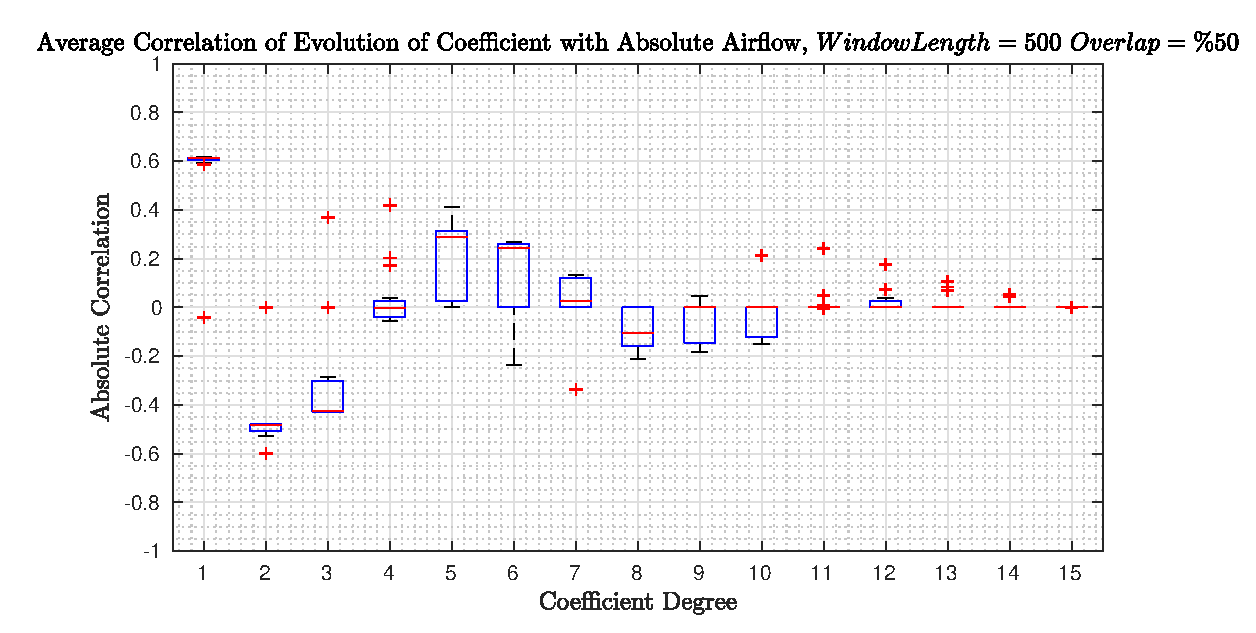
\includegraphics[width=\textwidth]{figures/corr_abs_coeff_for_degree_selection.eps}
		\caption{Boxplot for correlation coefficient of AR coefficient evolution with absolute value of airflow for different coefficient orders}
		\label{fig:absolute_airflow_window_coef}
	\end{center}
\end{figure}
\begin{figure}
	\begin{center}
		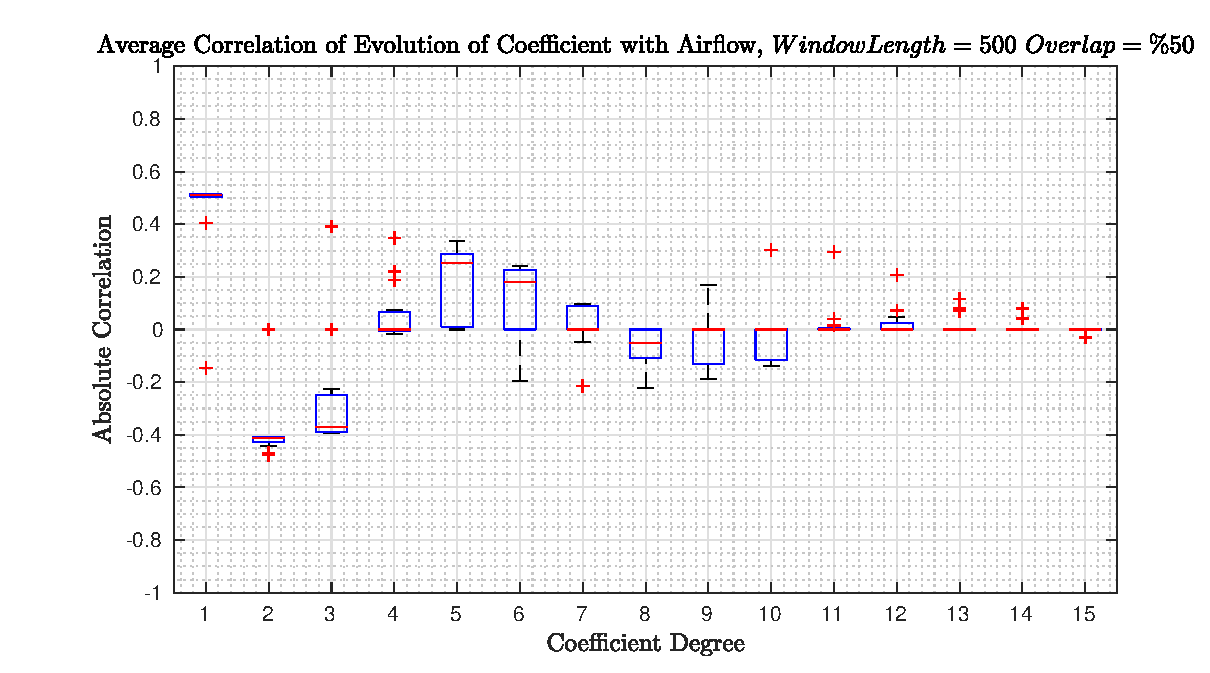
\includegraphics[width=\textwidth]{figures/corr_normal_coeff_for_degree_selection.eps}
		\caption{Boxplot for correlation coefficient of AR coefficient evolution with airflow for different coefficient orders}
		\label{fig:normal_airflow_window_coef}
	\end{center}
\end{figure}
\begin{figure}
	\begin{center}
		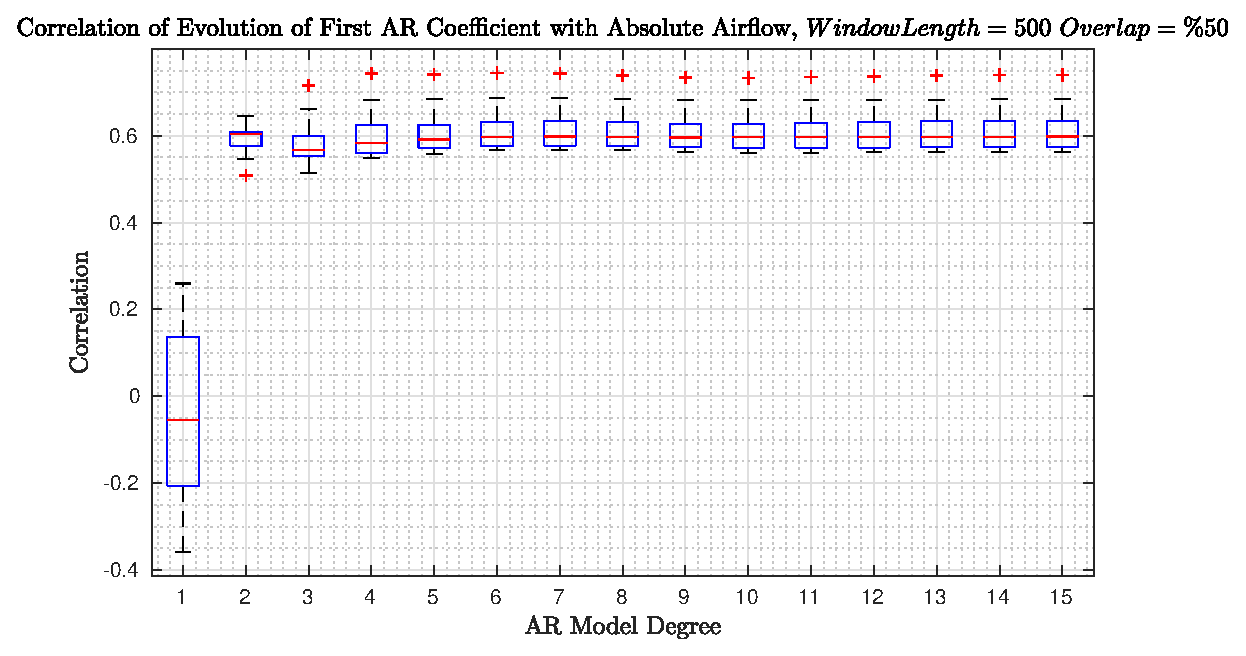
\includegraphics[width=\textwidth]{figures/corr_abs_for_ar_model_degree_selection.eps}
		\caption{Boxplot for correlation coefficient of AR coefficient evolution with airflow for different AR model orders}
		\label{fig:abs_airflow_window_ar_model}
	\end{center}
\end{figure}
\begin{figure}
	\begin{center}
		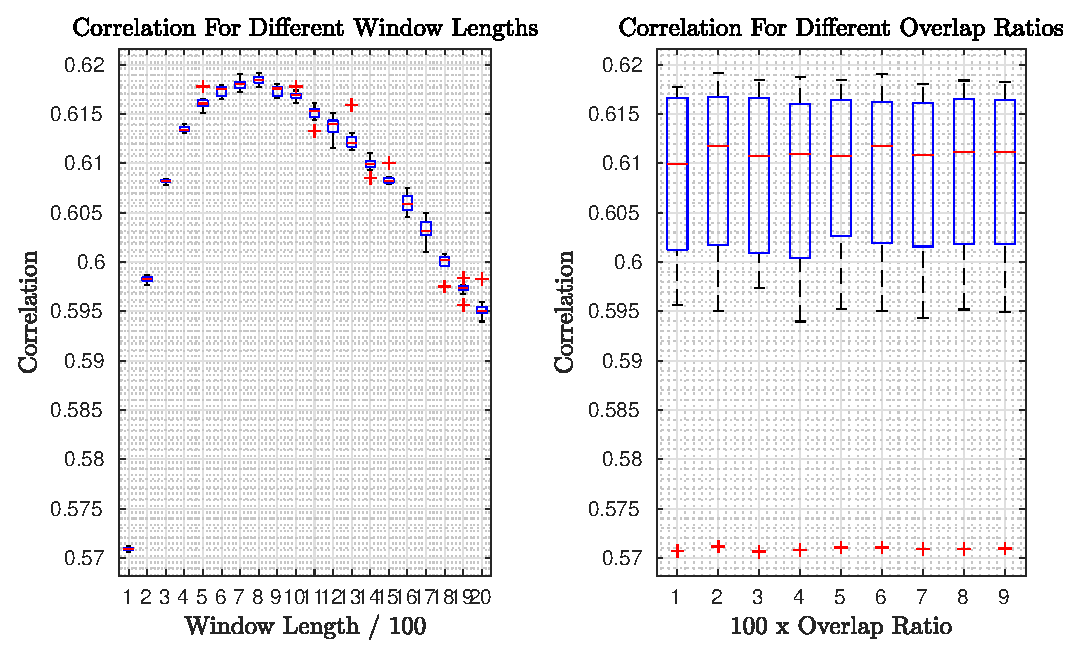
\includegraphics[width=\textwidth]{figures/corr_abs_for_window_length_selection.eps}
		\caption{Boxplot for correlation coefficient of first AR coefficient evolution with absolute airflow for different window lengths and overlap ratios}
		\label{fig:abs_airflow_window_ar_model_window_overlap}
	\end{center}
\end{figure}\par
The inference from figures  is that the correlation is decreasing with increasing coefficient order and the correlation with absolute value of flow is significantly greater. We will continue our analysis with absolute value of airflow for AR estimators. Now we will continue the analysis to find the best model order. For this, we run experiments with window length 500 and an overlap of \%50 with model orders from 1 to 15. The results are shown in figure \ref{fig:abs_airflow_window_ar_model}. As can be seen from figure, there isn't any significant difference after sixth order AR model, so we chose 6 as our model order. After selecting model order, the window length and overlap ratio are left to be decided on. In order to select them we run experiments with window lengths from 100 to 2000 with a seperation of 100 and overlap ratios from 10\% to 90\% with a separation of 10\%. The results for different window lengths and overlap ratios are summarized in figure \ref{fig:abs_airflow_window_ar_model_window_overlap}, according to the results best window length is 800 and difference in overlap ratio doesn't generate any difference in the correlation. We decided to use 90\% overlap to increase the resolution. \par
The resulting decision for univariate autoregressive solution with overlapping windows is 6, 800, 90\% for model order, window length and overlap ratio respectively. 
\subsection{Time Varying Autoregressive Model with Basis Functions}
The parameters for this method are model order, number of basis functions and the frequency difference in adjacent basis functions. \par 
First, we run experiments to determine the best model order and for this purpose run experiments with model orders from 1 to 15 where the number of basis functions are 201 (100 sines, 100 cosines and a constant) and the separation in frequency is 0.04 $Hz$. Experiment results are given in figure \ref{fig:abs_airflow_tvar_model_order}. Most correlation is achieved with the model order of 6 again. \par
After deciding on model order, we need to decide on number of basis functions and frequency separation of basis functions. Before doing this, we run experiments to determine the frequency coverage for best correlation and run experiments with separation of 0.025 $Hz$ and different number of basis frequencies from 50 to 300 with steps of 50. The result is given in figure \ref{fig:abs_airflow_tvar_freq_range}. According to test results 5 $Hz$ is enough to cover for best results.
\begin{figure}
	\begin{center}
		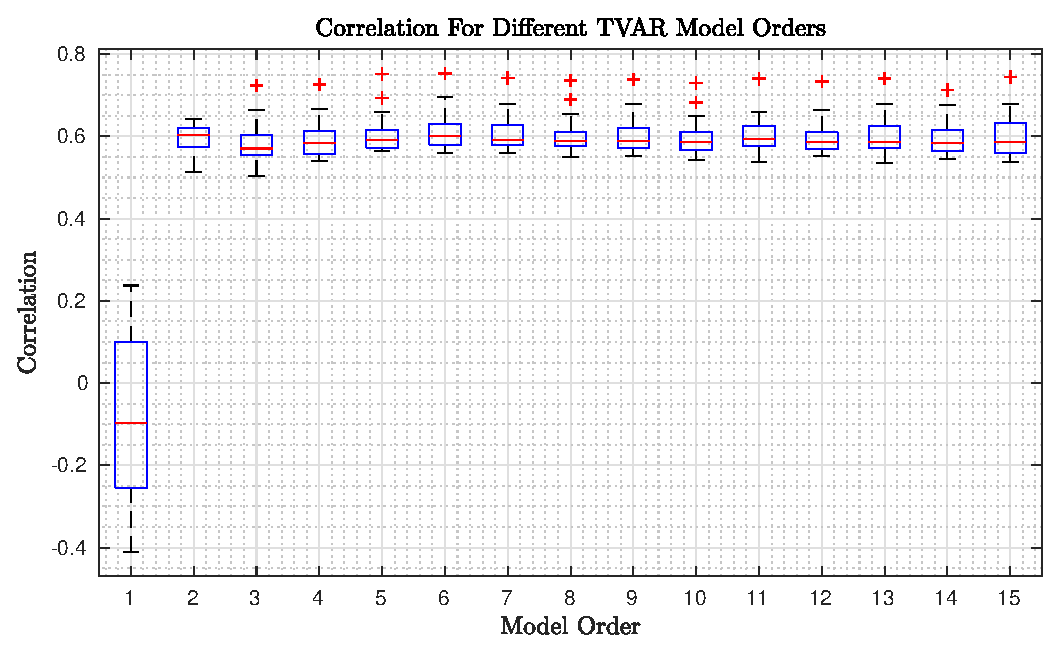
\includegraphics[width=\textwidth]{figures/corr_abs_for_tvar_ar_order_selection.eps}
		\caption{Boxplot for correlation coefficient of first AR coefficient evolution with absolute airflow for different TVAR model orders}
		\label{fig:abs_airflow_tvar_model_order}
	\end{center}
\end{figure}
\begin{figure}
	\begin{center}
		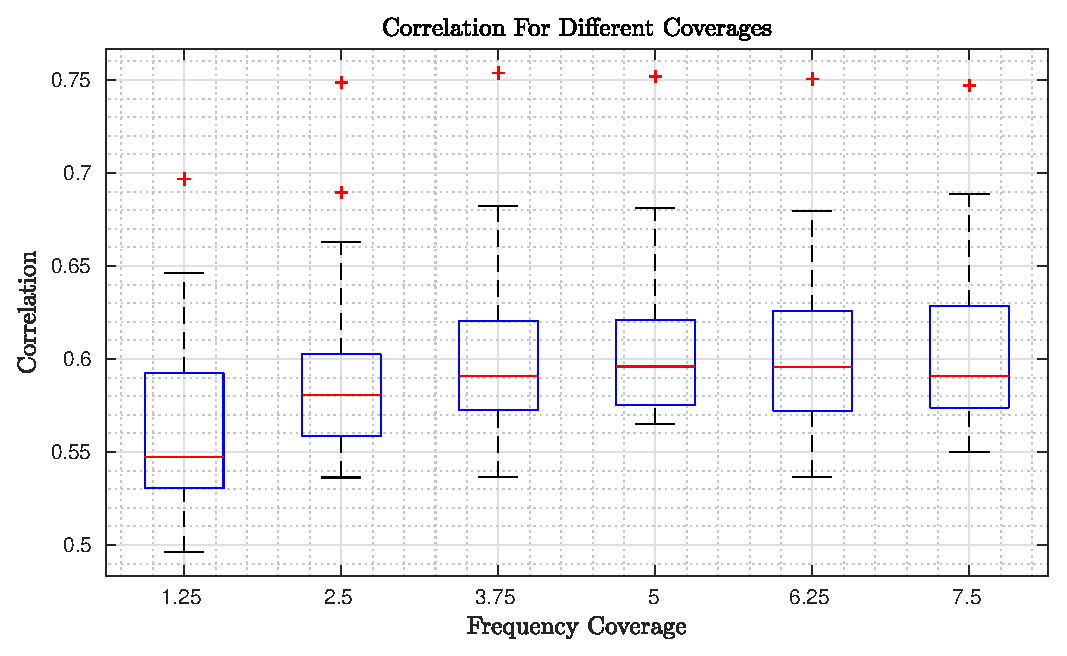
\includegraphics[width=\textwidth]{figures/corr_abs_for_tvar_frange_selection.eps}
		\caption{Boxplot for correlation coefficient of first AR coefficient evolution with absolute airflow for different frequency coverage}
		\label{fig:abs_airflow_tvar_freq_range}
	\end{center}
\end{figure}
Finally we run simulations to decide both the number of basis frequencies and frequency separation and for each tuning we covered the frequency range from 0 to 5 $Hz$. The results are given in figure \ref{fig:abs_airflow_tvar_numbasis_selection}, it shows that it doesn't make significant change to choose number of basis functions as 200 or 400. We chose it to be 250 for minimum standard deviation. \par 
To summarize, 6, 250, 0.02 is chosen for model order, number of basis frequencies and frequency separation respectively.
\begin{figure}
	\begin{center}
		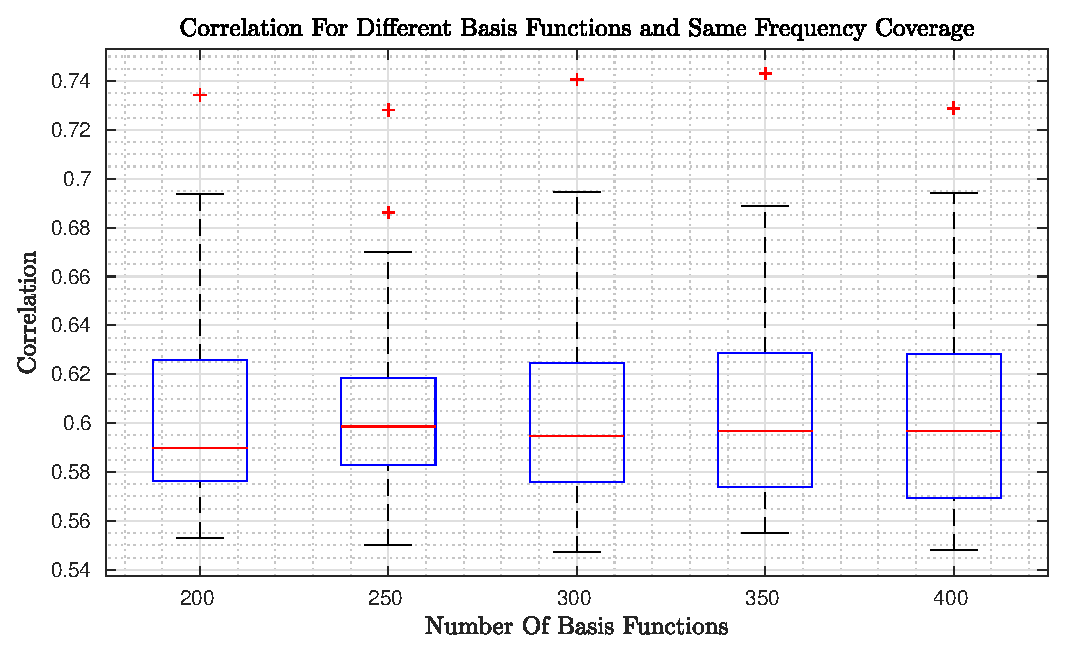
\includegraphics[width=\textwidth]{figures/corr_abs_for_tvar_numbasis_selection.eps}
		\caption{Boxplot for correlation coefficient of first AR coefficient evolution with absolute airflow for number of basis functions}
		\label{fig:abs_airflow_tvar_numbasis_selection}
	\end{center}
\end{figure} \par 

\subsection{Time Varying Autoregressive Model with Kalman Filter}
For this method, we used the noise estimated by windowing based AR modeling as the measurement noise variance, and look for the best noise variance for process noise. We run simulations where the state uncertainity goes from 0.0002 to 0.004 with steps of 0.0002. The results are given in \ref{fig:abs_airflow_kalman_noise_selection}. We chose 0.004 as our process variance.

\begin{figure}
	\begin{center}
		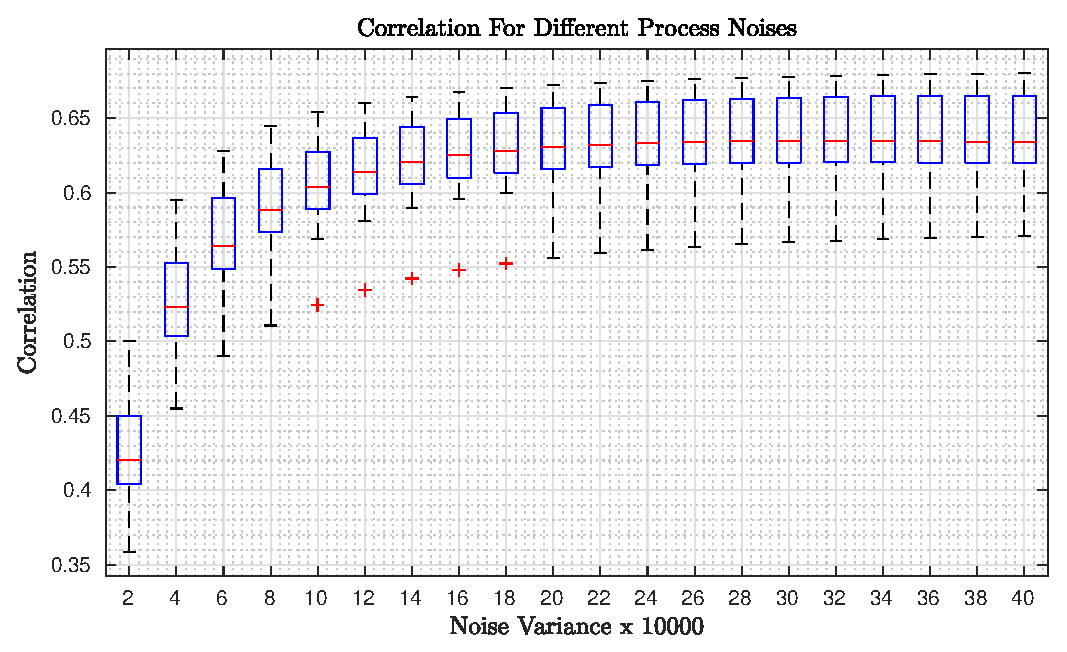
\includegraphics[width=\textwidth]{figures/corr_abs_for_kalman_noise_selection.eps}
		\caption{Boxplot for correlation coefficient of first AR coefficient evolution with absolute airflow for different process noise variances}
		\label{fig:abs_airflow_kalman_noise_selection}
	\end{center}
\end{figure}

\subsection{Short Time Fourier Transform}
\begin{figure}[h!]
	\begin{center}
		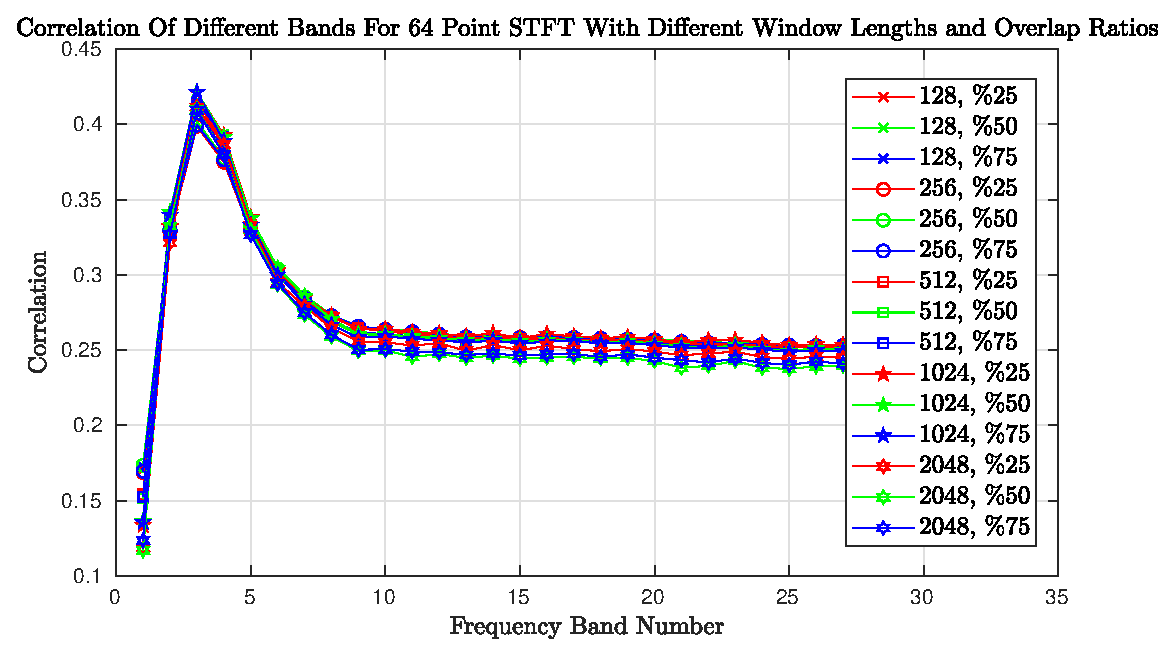
\includegraphics[width=\textwidth]{figures/corr_normal_for_stft_64.eps}
		\caption{Mean of correlations for each band for STFT method with 64 fft bins, window lengths and overlap ratios}
		\label{fig:airflow_stft_64}
	\end{center}
\end{figure}
\begin{figure}[h!]
	\begin{center}
		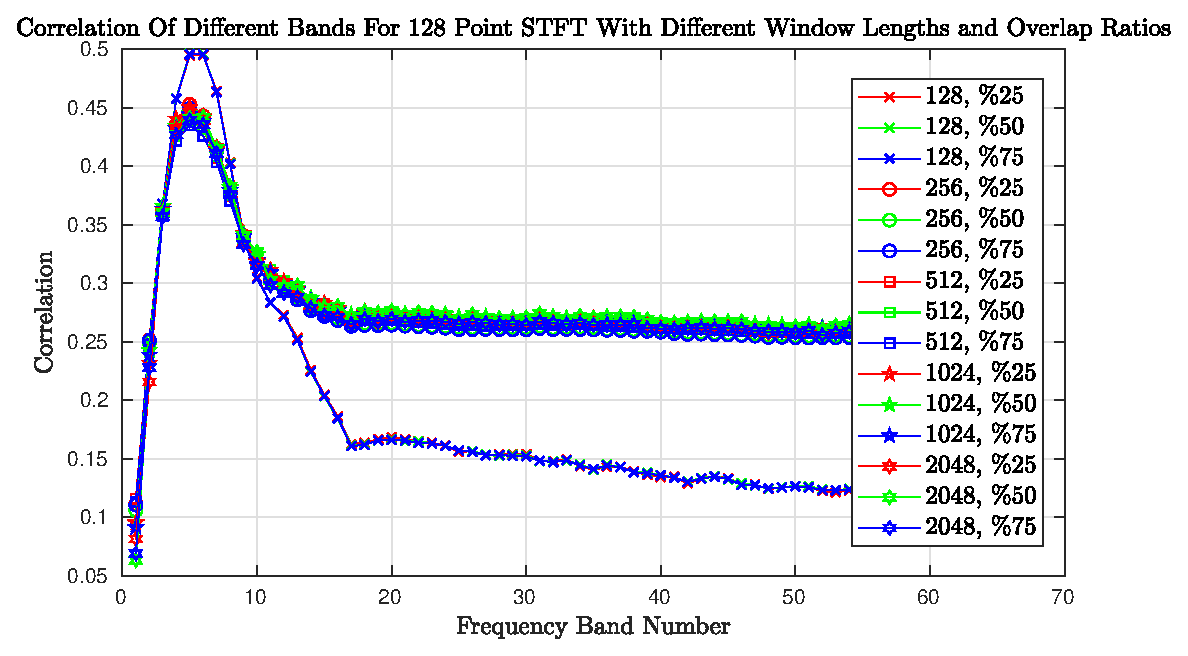
\includegraphics[width=\textwidth]{figures/corr_normal_for_stft_128.eps}
		\caption{Mean of correlations for each band for STFT method with 128 fft bins, window lengths and overlap ratios}
		\label{fig:airflow_stft_128}
	\end{center}
\end{figure}
\begin{figure}[h!]
	\begin{center}
		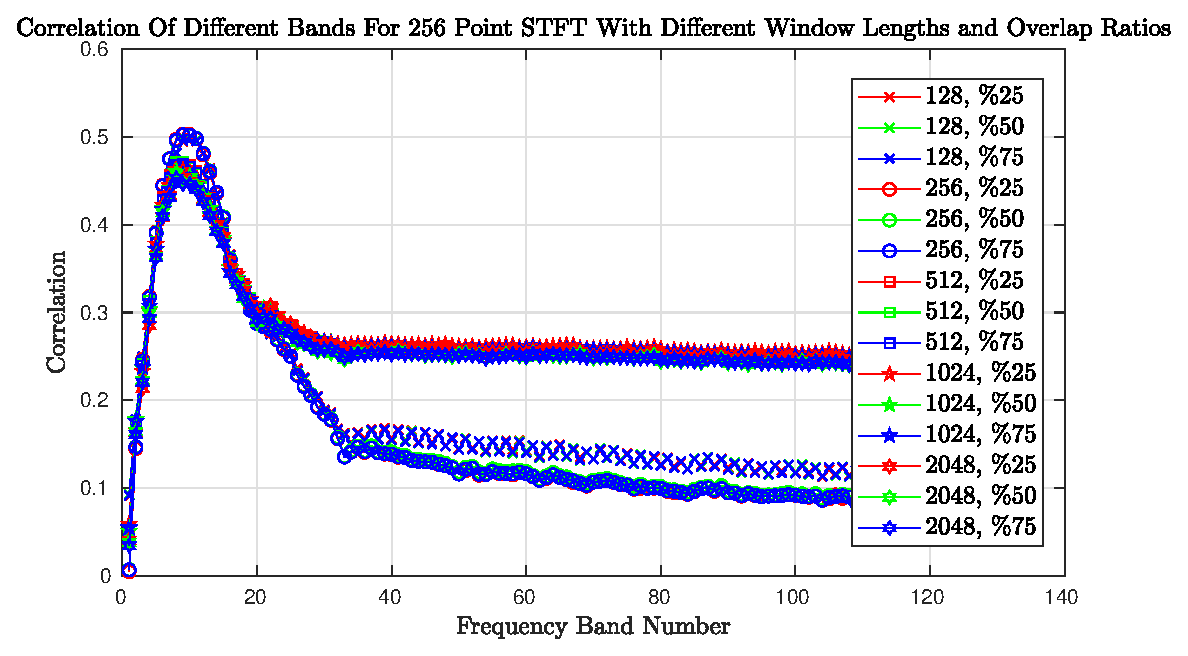
\includegraphics[width=\textwidth]{figures/corr_normal_for_stft_256.eps}
		\caption{Mean of correlations for each band for STFT method with 256 fft bins, window lengths and overlap ratios}
		\label{fig:airflow_stft_256}
	\end{center}
\end{figure}

\subsection{Unifying Estimations}
We run simulations with different number of vectors to be unified, where the vectors are outputs of univariate AR and STFT methods.
\begin{figure}[h!]
	\begin{center}
		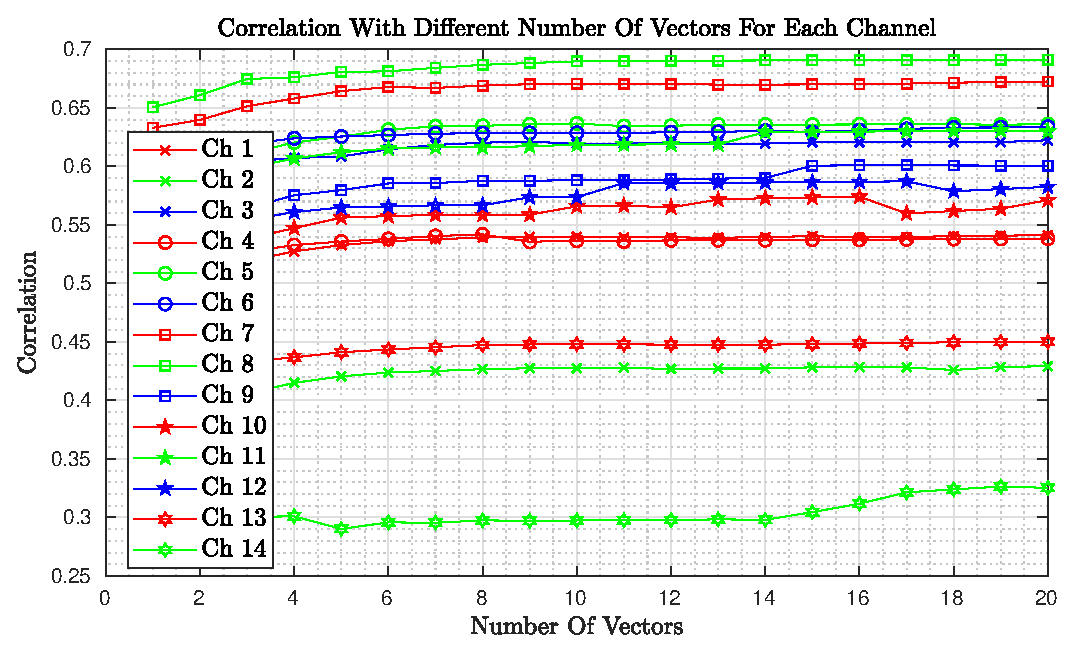
\includegraphics[width=\textwidth]{figures/corr_normal_unify.eps}
		\caption{Mean of correlations for each channel with different number of vectors unified}
		\label{fig:airflow_unify}
	\end{center}
\end{figure}
       

\subsection{Result}
\begin{table}[h!]
	\centering
	\begin{tabular}{|| c c c c ||} 
		\hline
		Channel & Univariate AR & Basis Functions & Kalman \\ [0.5ex] 
		\hline\hline
		1 & 0.6871 & 0.6862 & 0.6290 \\ 
		2 & 0.7440 & 0.7280 & 0.6802 \\
		3 & 0.6800 & 0.6699 & 0.6647 \\
		4 & 0.6310 & 0.6185 & 0.6536\\
		5 & 0.6153 & 0.6047 & 0.6649 \\
		6 & 0.5935 & 0.5963 & 0.6134 \\ 
		7 & 0.6031 & 0.6031 & 0.6328 \\ 
		8 & 0.5980 & 0.5885 & 0.6672 \\ 
		9 & 0.5761 & 0.5828 & 0.6351 \\ 
		10 & 0.5900 & 0.6009 & 0.6328 \\ 
		11 & 0.5681 & 0.5500 & 0.6197 \\ 
		12 & 0.5688 & 0.5719 & 0.6362 \\ 
		13 & 0.5733 & 0.5652 & 0.6127 \\ 
		14 & 0.5952 & 0.5916 & 0.5706 \\ 
		\hline
		\end{tabular}
		\caption{Correlation For Different Methods for All Channels}
		\label{table:1}
\end{table}
\chapter{AIRFLOW CURVE ESTIMATION}
\label{chapter:airflow-curve-estimation}
 

\section{Literature Review}
\section{Autoregressive Modeling}
In this chapter, we will analyze the respiratory sounds as if they are time varying autoregressive processes and try to find a correlation between time varying autoregressive coefficients and airflow over the mouth. 
We will look at three different methods for time varying autoregressive modeling of a signal after we give the description of autoregressive processes. Three methods are 
\begin{itemize}
	\item Windowing Based Autoregressive Modeling
	\item Time Varying Autoregressive Modeling with Basis Functions
	\item Time Varying Autoregressive Modeling with Particle Filters.
\end{itemize}
\subsection{Description of Autoregressive Processes}
Autoregressive process is a class of discrete random processes whose output at a time can be written with a fixed combination of number of past values plus a sample from a white Gaussian noise. It can be formulated as in \ref{AR formula}. The $a_{i}$'s are the AR coefficients, $N$ is the order of process and $e$ is the noise term which has a constant variance. 
\begin{equation}\label{AR formula}
x(n) = \sum_{i=1}^{N}{a_ix(n-i)} + e(n) 
\end{equation}
An autoregressive process is equivalent to a infinite impulse response filter whose input is white Gaussian noise. 
Autoregressive processes are widely used in many areas, including economics, statistics and signal processing. In general, and in this thesis too, the processes used for analysis purposes are assumed to be stationarity.
\subsubsection{Mean, Variance and Autocorrelation Of Autoregressive Processes}
Expectation is a linear operator, then we can write the equation \ref{Mean of AR}. Recalling that e is white Gaussian i.e. $\mu_e=0$ at least one of the followings must hold $\sum_{i=1}^{N}a_i = 1$ or $\mu_X = 0$. For variance, one can write the \ref{Variance of AR -1}. Since white noise is uncorrelated with the values of process, the last term is zero. However, the middle term is a finite, nonzero value. This implies $\sum_{i=1}^{N}a_i < 1$. 
\begin{equation}\label{Mean of AR}
\mu_X = \sum_{i=1}^{N}{a_i\mu_X} + \mu_e 
\end{equation}
\begin{equation}\label{Variance of AR -1}
\sigma_{X}^2 = \sum_{i=1}^{N}{a_i\sigma_X^2} + \sigma_e^2 + 2\sigma_{Xe} 
\end{equation}
If we reorganize what we have from deductions we had while calculating mean and variance, we can list as following:
\begin{itemize}
	\item $\sum_{i=1}^{N}a_i = 1$ or $\mu_X = 0$, from mean
	\item $\sum_{i=1}^{N}a_i < 1$, from variance
\end{itemize}
Now we can say that $\sum_{i=1}^{N}a_i < 1$ is needed for an autoregressive process to be at least wide sense stationary and the mean of an autoregressive process must be zero.\linebreak
In order to look at autocorrelation, let's first rewrite the variance equation as in \ref{Variance of AR}, \ref{Variance of AR 1} and \ref{Variance of AR 2}.
\begin{equation}\label{Variance of AR}
\sigma_{X}^2 = E(X(n)X(n)) - \mu_{X}^2 
\end{equation}
\begin{equation}\label{Variance of AR 1}
\sigma_{X}^2 = \sum_{i=1}^{N}a_iE(X_nX_{n-i}) + E(X_ne_n) - \mu_{X}^2 
\end{equation}
\begin{equation}\label{Variance of AR 2}
\sigma_{X}^2 = \sum_{i=1}^{N}a_iR_{XX}(i) + \sigma_e^2
\end{equation}
One of the descriptive functions of random processes is autocorrelation function given in \ref{Autocorrelation}. If we rewrite X(n) as in \ref{AR formula} we can conclude in a recursive equation for autocorrelation function as in \ref{YuleWalker 1}. The equations in \ref{YuleWalker 1} are called "Yule-Walker Equations".
\begin{equation}\label{Autocorrelation}
r_{XX}(k) = \frac{E[X(n-k)X(n)]}{\sigma_X^2}
\end{equation}
\begin{equation}\label{YuleWalker 1}
r_{XX}(0) = 1,\qquad 
r_{XX}(k) = \sum_{i=1}^{N}{a_ir_{XX}(k-i)}, \qquad k \geq 1
\end{equation}
This leads to a difference equation which can be expressed with vector equations as in \ref{yulewalker matrix 1}.
\begin{equation}\label{yulewalker matrix 1}
\begin{pmatrix}
r_{XX}(1) \\ 
r_{XX}(2) \\ 
\vdots \\ 
r_{XX}(N-1)\\ 
r_{XX}(N) 
\end{pmatrix} =  
\begin{pmatrix}
1 & r_{XX}(1) & ... & r_{XX}(N-2) & r_{XX}(N-1) \\
r_{XX}(1) & 1 & ... & ... & r_{XX}(N-2) \\
\vdots    & \vdots    & \vdots & \vdots & \vdots \\
r_{XX}(N-2) & ... & ... & 1 & r_{XX}(1) \\
r_{XX}(N-1) & r_{XX}(N-2) & ... & r_{XX}(1) & 1
\end{pmatrix} 
\begin{pmatrix} 
a_{1} \\ 
a_{2} \\
\vdots \\
a_{N-1} \\
a_{N} \end{pmatrix}
\end{equation}
\subsection{Description Of Time Varying Autoregressive Processes}
Time varying autoregressive process is defined in \ref{TVAR formula}. In this model, AR coefficients are dependent on time. This model is very useful for applications where signals are not stationary. 
\begin{equation}\label{TVAR formula}
x(n) = \sum_{i=1}^{N}{a_i(n)x(n-i)} + e(n) 
\end{equation}
\subsection{Autoregressive Modeling With Windows}
This method divides the signal into parts and finds the autoregressive coefficients by a well known method such as Yule-Walker or Burg or direct matrix inversion. The important thing to note is the divided parts are assumed to be stationary. The method is given in algorithm \ref{Windowed AR}.
\begin{algorithm}
	\caption{AR Coefficients Estimation With Overlapping Windows}
	\label{Windowed AR}
	\begin{algorithmic}[1]
		\Procedure{WindowedAR}{signal, order, windowLength, overlap}
			\State $windowStart \gets 1$
			\State $L \gets Length(signal)$
			\State $lastWindowStart \gets {L-windowLength}$
			\While{$windowStart \leq lastWindowStart$}
				\State $temp \gets signal(windowStart:(windowStart+windowLength))$
				\State $AR(:,i) \gets EstimateAR(temp, N)$
				\State $windowStart \gets windowStart + windowLength$
			\EndWhile
		\State \textbf{return} $AR$
		\EndProcedure
	\end{algorithmic}
\end{algorithm}\\
\newline
There are several methods to estimate the AR coefficients of given signal. Yule Walker Method, Burg's Method, Least Squares are the well known methods. Usually Yule Walker approach is used, however it is reported that Yule-Walker method fails where the autocovariance matrix is poorly conditioned and least squares approach doesn't guarantee the estimated autoregressive model to be stable, we used Burg's method to estimate autoregressive coefficients [Wharton Statistics].

To test the relation between ar coefficients and flow, we looked at the correlation between the AR coefficients of overlapping windows and down sampled version of flow. We also looked at the correlation between AR coefficients and absolute value of flow. The absolute value of correlation between downsampled version of flow and array of estimated AR coefficients for different model and coefficient orders is given in figures \ref{winArNormalCorr} and \ref{winArAbsCorr}. Third channel is chosen randomly for this analysis.
\begin{figure}[H]
	\centering
	\includegraphics[width=0.7\linewidth]{windowAr_NormalOrders.eps}
	\caption{Absolute Correlation Between Flow and AR Coefficients for Different Model and Coefficient Orders}
	\label{winArNormalCorr}
\end{figure}
\begin{figure}[H]
	\centering
	\includegraphics[width=0.7\linewidth]{windowAr_AbsOrders.eps}
	\caption{Absolute Correlation Between Absolute Flow and AR Coefficients for Different Model and Coefficient Orders}
	\label{winArAbsCorr}
\end{figure}

It can be concluded that the greatest correlation is observed for the first AR coefficient in both cases and the correlation with absolute value of flow is greater. It is seen that the correlation increases with model order however it doesn't increase significantly after a point. To find this point, we plot the correlation of absolute flow with first AR coefficient for different model orders in figure \ref{winArAbsFirst}. In the boxplot graph, each box consists of 14 values, each is the average of corresponding channel calculated over 25 subjects. The graph showing the ratio of mean of correlation to variance of correlation is given in By looking at figures \ref{winArAbsFirst} and \ref{winArAbsFirstMeanVar}, we decided to use 6 as our model order for further analysis.
\begin{figure}[H]
	\centering
	\includegraphics[width=0.8\linewidth]{windowAr_AbsFirst.eps}
	\caption{Average Correlation Between Absolute Flow and First AR Coefficient for Different Model Orders}
	\label{winArAbsFirst}
\end{figure}
\begin{figure}[H]
	\centering
	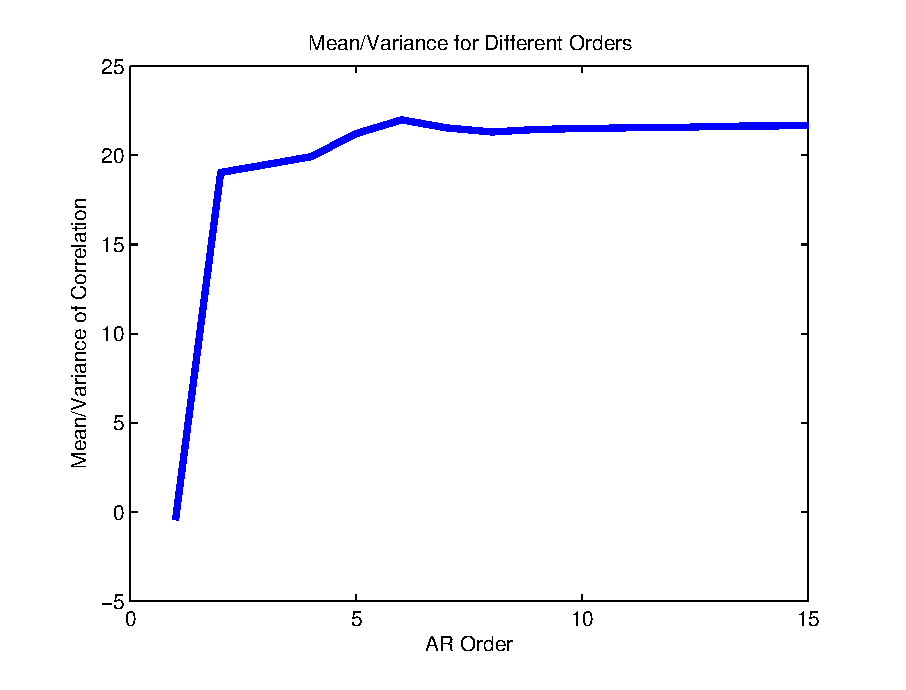
\includegraphics[width=0.8\linewidth]{windowedAr_MeanOverVarForOrders.eps}
	\caption{Ratio Of Correlation Mean To Correlation Variance for Different Orders}
	\label{winArAbsFirstMeanVar}
\end{figure}


After setting model order to 6, we run tests to choose the window length and overlap ratio pair giving the best correlation. The resulting graph is given in figure \ref{winArWinLenOverlap}. From the figure, one can say that window length must be greater than 400 and must not exceed 1200 and overlap is not making a lot of difference. This makes sense because the correlation is calculated with the decimated versions of flow, in other words increasing the overlap ratio increases the resolution.  

After deciding AR order, window length and overlap, we run tests to find the optimum post filtering setup. To test this, we passed the estimation through butterworth filters with different cutoff frequency and orders. We reached the figure \ref{winArCutoffOrder} for different orders and cutoff frequencies.
\begin{figure}[H]
	\centering
	\includegraphics[width=0.8\linewidth]{windowAr_WinLenOverlap.eps}
	\caption{Average Correlation Between Absolute Flow and First AR Coefficient for Different Window Lengths and Overlaps}
	\label{winArWinLenOverlap}
\end{figure}

 

\begin{figure}[H]
	\centering
	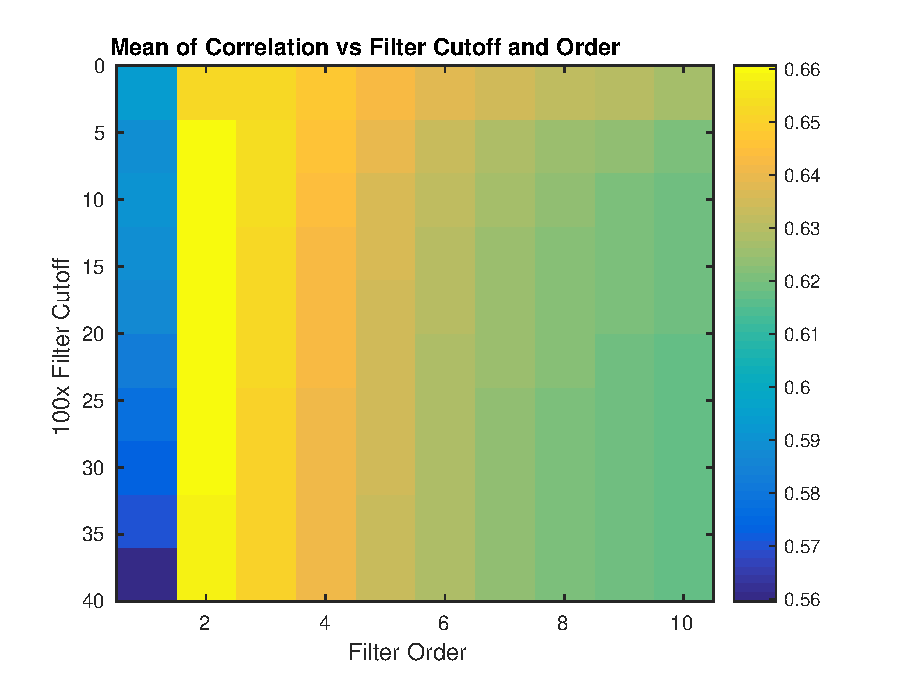
\includegraphics[width=0.8\linewidth]{windowedArCutoffOrder.eps}
	\caption{Average Correlation For Different Filter Cutoff and Orders}
	\label{winArCutoffOrder}
\end{figure}

\section{Time Varying Autoregressive Modeling}
Time varying auto regressive (TVAR) modelling is widely used in nonstationary signal analysis. TVAR is also used to analyze respiratory sounds. It is reported in [Koray, SİU] a good correlation is achieved with first TVAR coefficients and absolute value of flow curve. In this thesis, we will go over two approaches for this modeling. The first one is using combinations of Fourier basis functions for coefficients, the second one is using particle filters.  
The equation defining a TVAR process is given in \eqref{TVAR formula}. As the name suggests, AR coefficients are changing over time.

\subsection{Fourier Basis Functions}
One of the methods for TVAR coefficient estimation is using Fourier basis functions. This method rely on the assumption that the coefficients to be estimated have some periodicity. 
Using Fourier basis functions for airflow is based on the assumption that airflows are mostly periodic and one can approximate them by a linear combination of sine and cosine waves.
\subsubsection{Method}
The assumption can be formulated as in \eqref{Coefficient Basis}. Each coefficient is a linear combination of $K$ basis functions with constant weights $b_j$
\begin{equation}\label{Coefficient Basis}
a_{i}(n) = \sum_{j=1}^{K}{a_{ij}u_{j}(n-i)}
\end{equation}
By rewriting \eqref{TVAR formula} using \eqref{Coefficient Basis} for coefficients, we can end up in 
\begin{equation}\label{TVAR formula_2}
x(n) = \sum_{i=1}^{N}\sum_{j=1}^{K}{a_{ij}u_j(n-i)x(n-i)} + e(n) 
\end{equation}

\subsubsection{Tests and Results}

\subsection{Particle Filtering}
\subsubsection{Method}
\subsubsection{Tests and Results}

%\subsection{Kalman Filtering - Smoothing}
%\subsubsection{Method}
%\subsubsection{Tests and Results}

\section{Time - Frequency Analysis}
\subsection{Method}
\subsection{Tests and Results}

\section{Unifying Estimations}
\subsection{Method}
\subsection{Tests and Results}


\chapter{AIRFLOW PHASE DETECTION}
\label{chapter:introduction}
Start with an introduction...

\section{Estimation of Periods}
\section{Estimation of Change Point Locations}
\section{Feature Extraction}
\section{Results}

\chapter{CONCLUSION}
\label{chapter:conclusion}

The conclusions of the thesis should come
here.
% \nocite{NewEntry1,NewEntry2,NewEntry3,NewEntry4,NewEntry5,
% NewEntry6,
% NewEntry7,NewEntry8,NewEntry9,NewEntry10,NewEntry11,NewEntry12}

%\cite{*}
\bibliographystyle{styles/fbe_tez_v11}
\bibliography{references}

\appendix
\chapter{APPLICATION}
The appendices start here.

\end{document}